\section{Evaluation}
\label{sec:evaluation}

In this section, we quantify the benefits of using a wireless mesh in crowd-shared home networks for public Internet access. In Section \ref{evaluation:environment}, we present the simulation environment, the modeling of router on/off periods, and the metrics used to evaluate the efficiency of the wireless mesh. Section \ref{evaluation:results} provides a comparative study of crowd-shared home networks with and without a wireless mesh based on our simulation results.

\subsection{Simulation Environment}
\label{evaluation:environment}

Using python, we developed a simulator that models the behaviour of guests flows in a crowd-shared network connected through a wireless mesh network. The simulator uses TFA wireless mesh topology [] which consists of 21 nodes. In our simulator, each TFA node represents an access home router which shares 8 Mbps of its internet access capacity, whereas each mesh link has the capacity a IEEE 802.11ac wireless link with 40 Mhz bandwidth and 200 Mbps data rate. 

To model the sharing policy of the access routers owners, the simulator switches the router ON and OFF for different time periods during the simulation lifetime. The length of the ON and OFF period are randomly generated out of an exponential distribution with two different mean values (555 mintues for OFF period and 106 minutes for the ON period). The mean values are driven from real world data of home routers owners behaviour. To keep track of the ON and OFF period, the simulator equips each router with a timer which expires at the end of an ON/OFF period. The simulator distinguishes between ON and OFF status of a router by using a flag for each router which is true when the router is ON and False when the router is OFF. 

To reflect real world traffic, we consider dynamic communication pattern where guests flows arrive to and departure from the network at certain time points. Flows arrival rates and durations are generated randomly based on Poisson and exponential distribution, respectively. Each flow has constant bit rate which is sampled out of a uniform distribution. Since in reality the flows load across the home routers may differ due to the number of guests connected to each router, we use geometric distribution to randomly choose at which router the next flow will arrive. 

To grant internet access to the flows, the simulator implements two methods. The first method only give access to flows through the router at which they arrive given that there is enough internet access capacity. This method ignores the mesh network. On the other hand, the second method considers the mesh network by redirecting flows which does not fit in the local access routers to other routers through the mesh network. The router to which the flow is redirected are selected using worst-fit decreasing algorithm. The algorithm starts by sorting the flows to be redirected in non-decreasing order of their rates. Then, for each flow (starting with the flow with the highest rate), the algorithm selects the router with the highest available internet access capacity which fits the flow rate. The shortest path between the router is chosen based on the number of hops. The worst-fit decreasing algorithm is also used to redirect flows when a router goes OFF. This sustains as much as possible flows in the network and reduce disruption by the routers owners sharing policy.
%Furthermore, to show performance of the system under dynamic communication pattern, we consider flows with limited life time which arrive and leave the system at certain time point.   

The simulation proceeds in discrete time ticks. At each time tick, the simulator updates the ON/OFF timer of the access routers and subsequently switches the routers with expired timer ON or OFF depending on their current status. It also removes flows which expires and generates new flows if required. Furthermore, it assigns flows to home access routers either without considering the mesh network (method 1) or with the mesh network (method 2). When the mesh network is considered, the simulator also updates the available capacity of the mesh links through which the flows are redirected. 

To evaluate the benefits of mesh network, we measure the average shared bandwidth utilization of the access router as well as the accumulated acceptance rate of the network at each time tick. At time tick $t$, we define \emph{the accumulated acceptance rate= the total rates of flows finished up to $t$ / (the total rates of flows finished up to $t$ + total rates of flows rejected up to $t$)}.
%${the accumulated acceptance rate =\displaystyle \frac{the\ total\ rates\ of\ flows\ finished\ up\ to\ t} {(the total rates of flows finished up to t + total rates of rejected flows up to t)}}$. 
From the acceptance rate, we exclude the flows which are still running and may finish in the future. 

Due to the large mean values of the ON and OFF period (8 hours OFF and 1.5 hours ON), we run each simulation for 60 hours with time scale of 20 minutes. We perform 20 runs and report the average. 


\begin{figure}[h]
\begin{center}
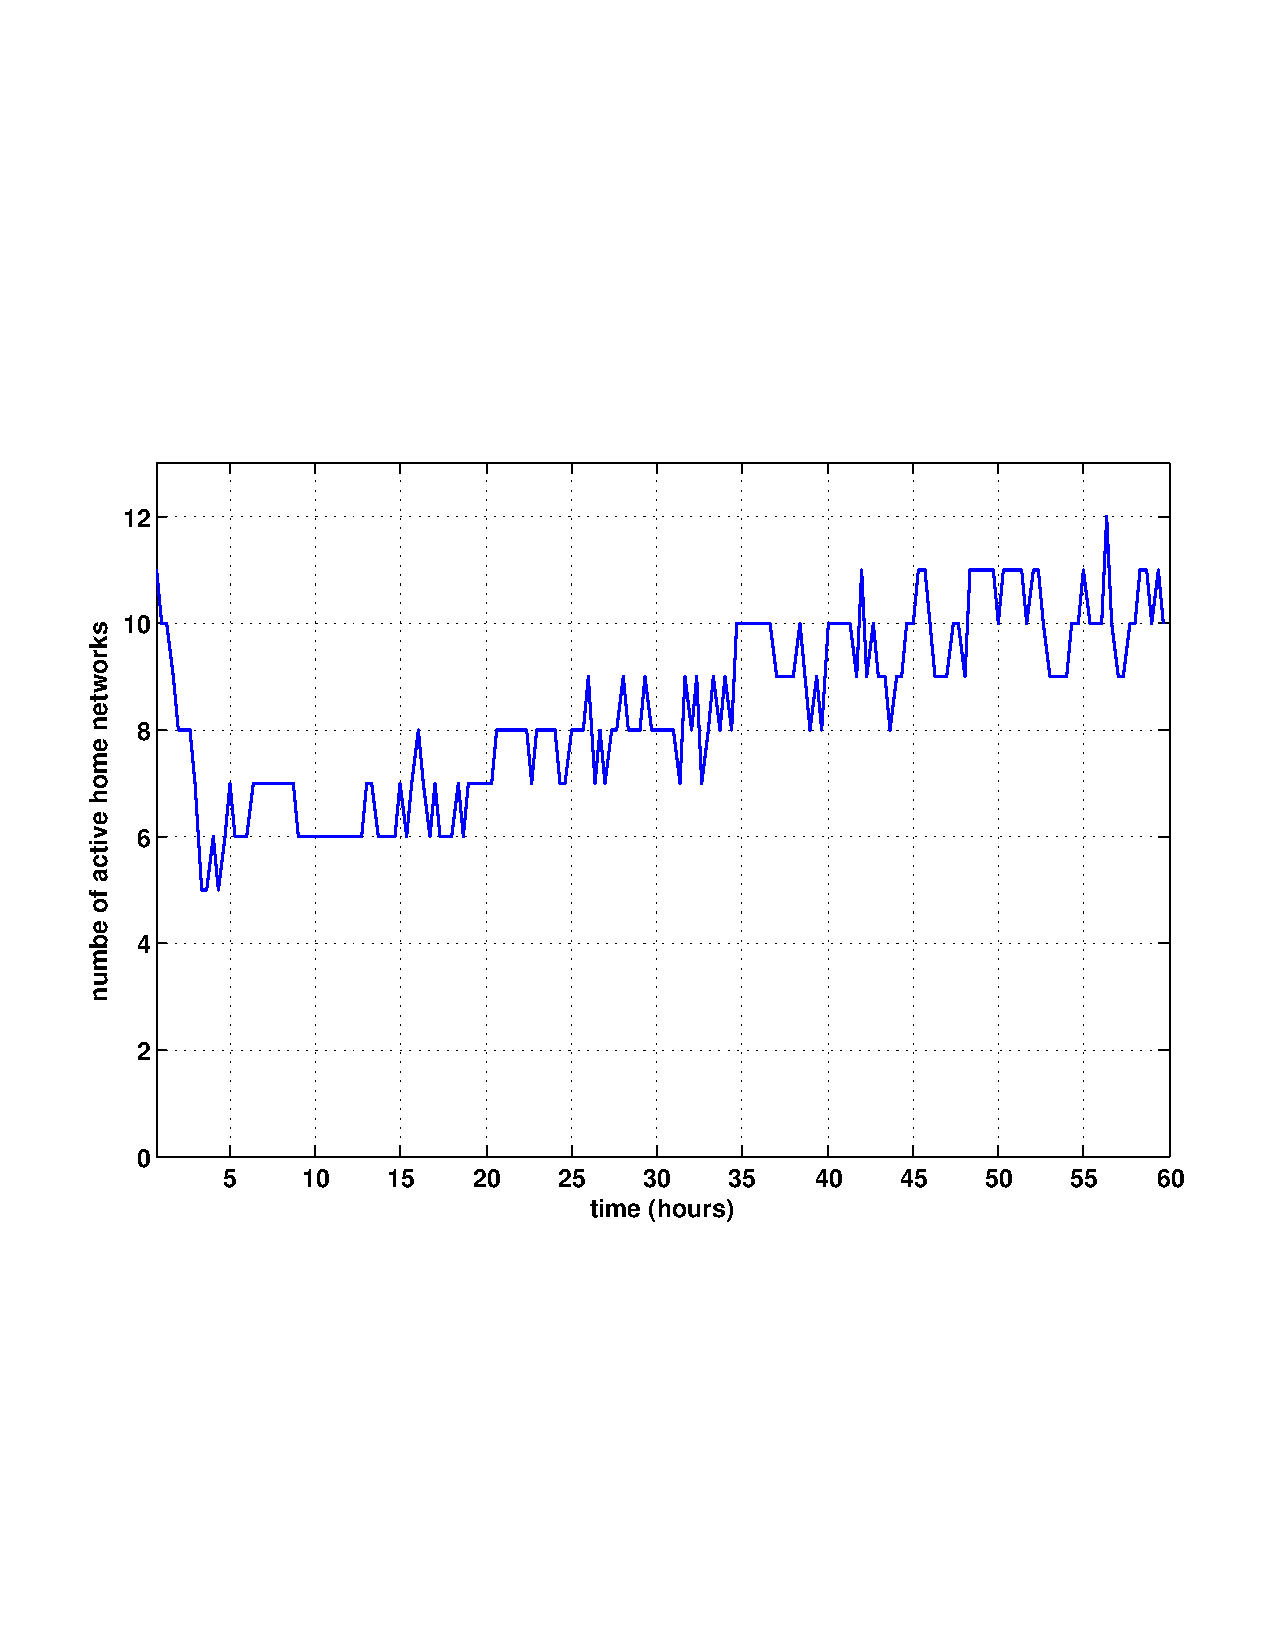
\includegraphics[width=1\linewidth]{../../results/simulation/on_routers2.pdf}  
\caption{Number of active home routers.}
\label{fig:active_routers}
\end{center}
\end{figure}


\subsection{Simulation Results}
\label{evaluation:results}

Initially, we measure the shared bandwidth utilization and request acceptance rate with an arrival rate of 50 flows per minute over a 60-hour period. Fig. \ref{fig:utilization} illustrates a low utilization of the shared bandwidth without a wireles mesh during the whole period, although there is high demand for Internet access by guest users attached to the various home networks. In contrast, a wireless mesh allows to capitilize the unused capacity and accommodate a larger volume of guest user traffic. More precisely, according to Fig. \ref{fig:utilization} guest user traffic redirection through the wireless mesh results in the full utilization of the bandwidth shared by home network users. Furthermore, crowd-shared home networks with a wireless mesh can accommodate substantially higher guest user traffic, as depicted in Fig. \ref{fig:acceptance}. This stems from the high utilization of the shared bandwidth. 

\begin{figure}[h]
\begin{center}
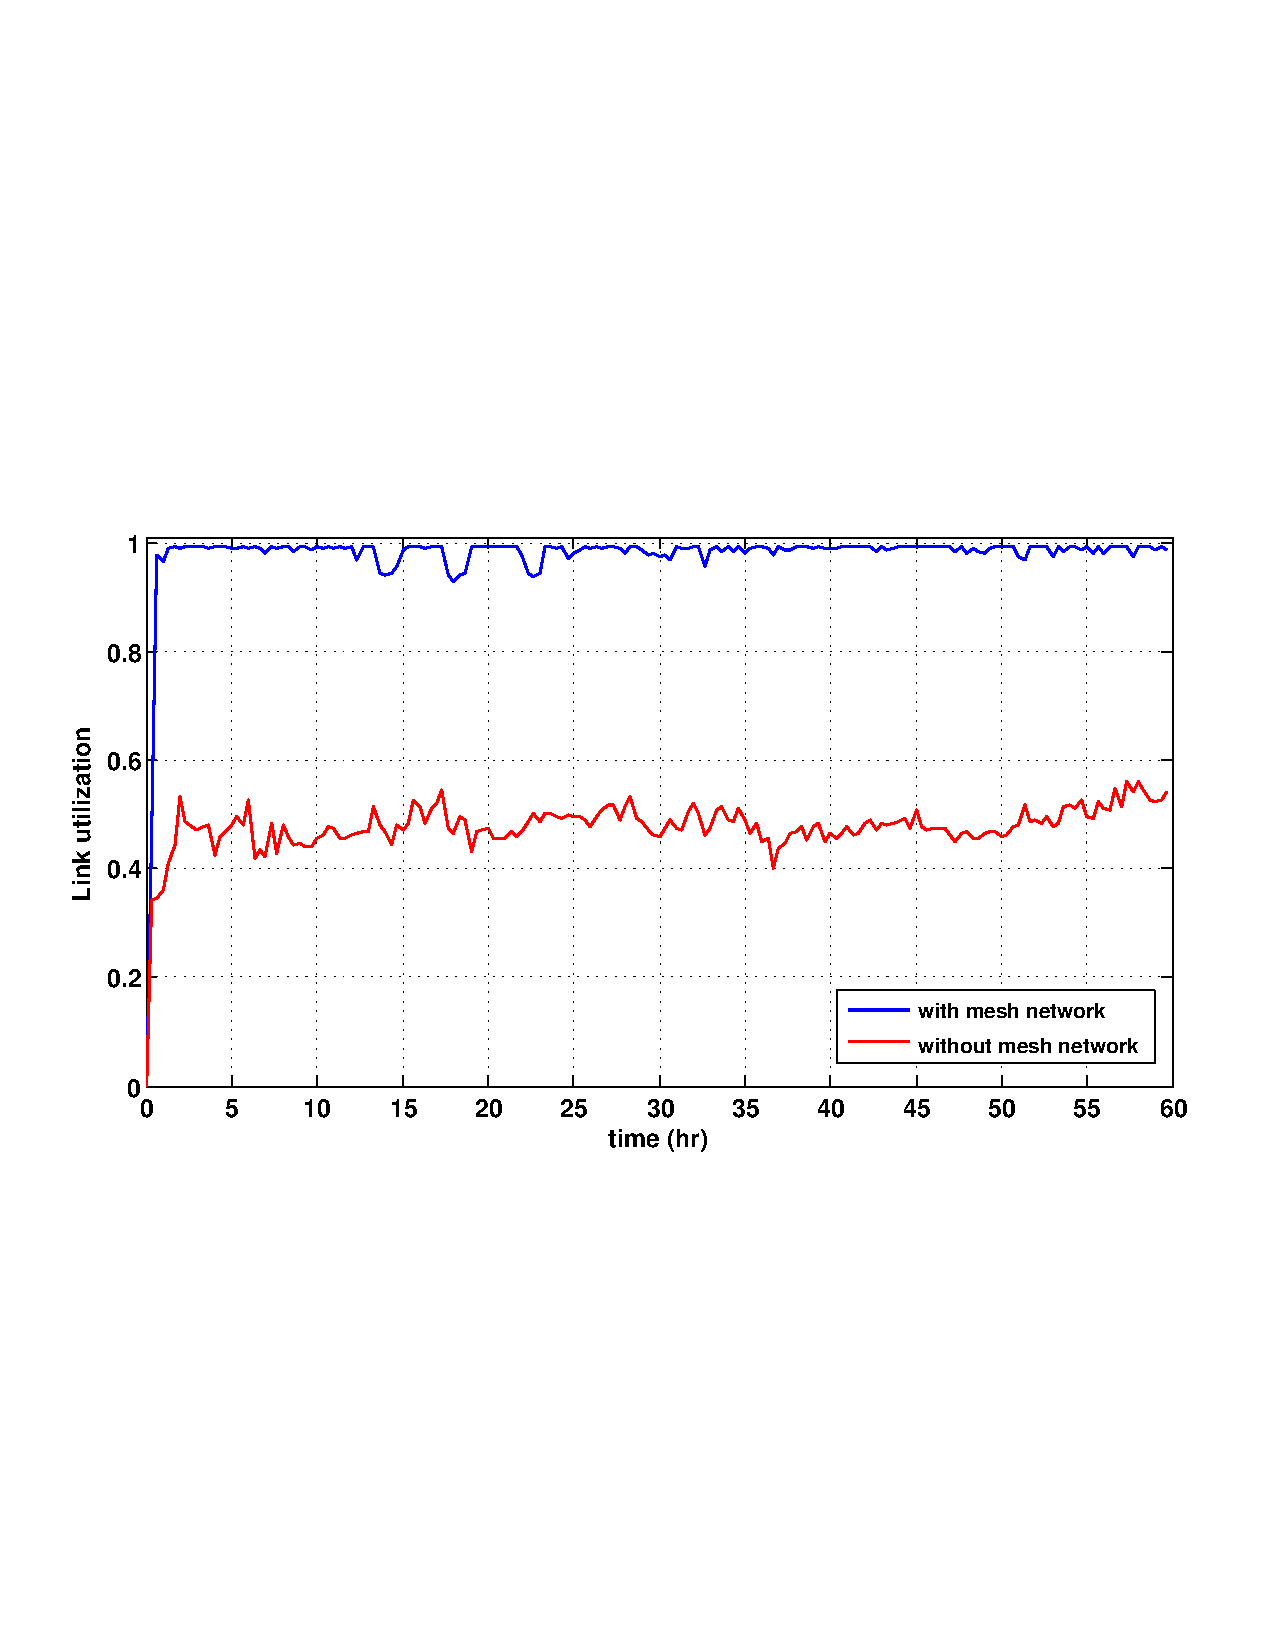
\includegraphics[width=1\linewidth]{../../results/simulation/utilization.pdf}  
\caption{Shared bandwidth utilization.}
\label{fig:utilization}
\end{center}
\end{figure}

\begin{figure}[h]
\begin{center}
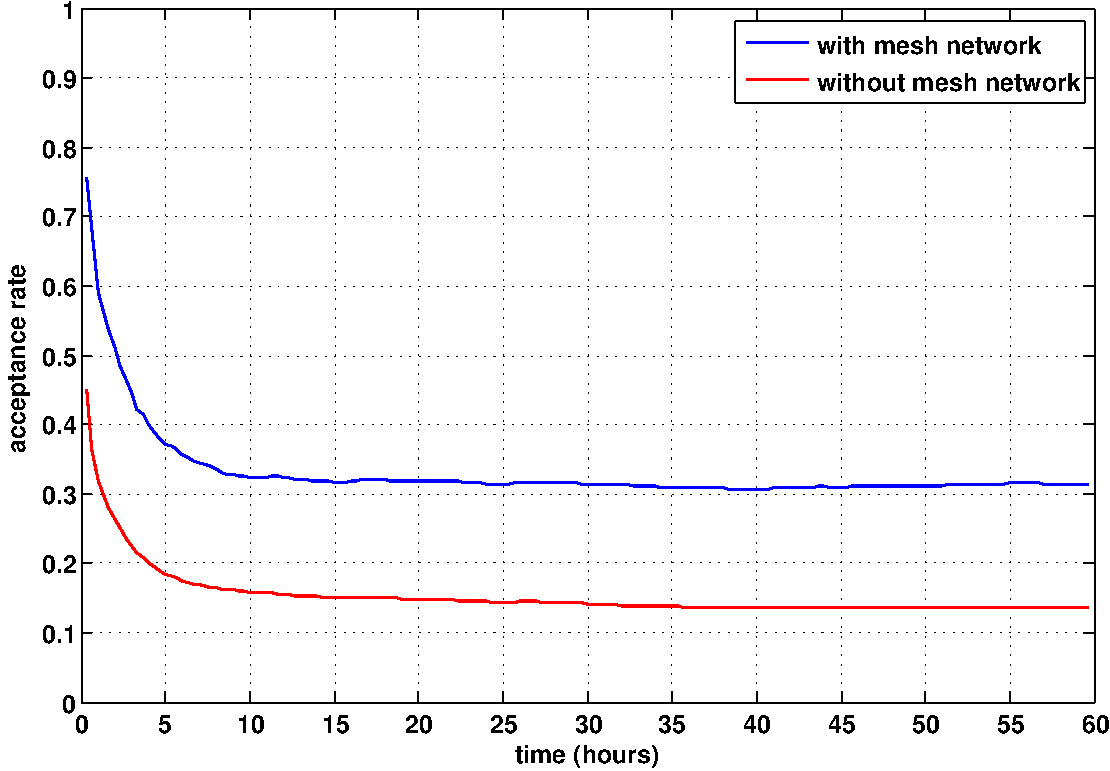
\includegraphics[width=1\linewidth]{../../results/simulation/acceptance_rate.pdf}  
\caption{Guest user traffic acceptance rate.}
\label{fig:acceptance}
\end{center}
\end{figure}

We further measure the shared bandwidth utilization with a wide range of guest user traffic demands. In this respect, Fig. \ref{fig:acceptance} illustrates the shared bandwidth utilization with diverse flow arrival rates, ranging from 10 to 100 flows per minute. This simulation result corroborates the efficiency of the wireless mesh for various traffic loads, as the shared bandwidth utilization always remains very high. Without the presence of a wireless mesh, Fig. \ref{fig:acceptance} shows poor bandwidth utilization, especially with low guest user traffic demand. In this particular case, the inability to redirect guest user traffic to home networks with available bandwidth results in wasting most of the shared bandwidth. Eventually, our simulation results show the significant benefit that a wireless mesh can bring in crowd-shared home networks, by effectively pooling shared resources across the interconnected home networks. 

\begin{figure}[h]
\begin{center}
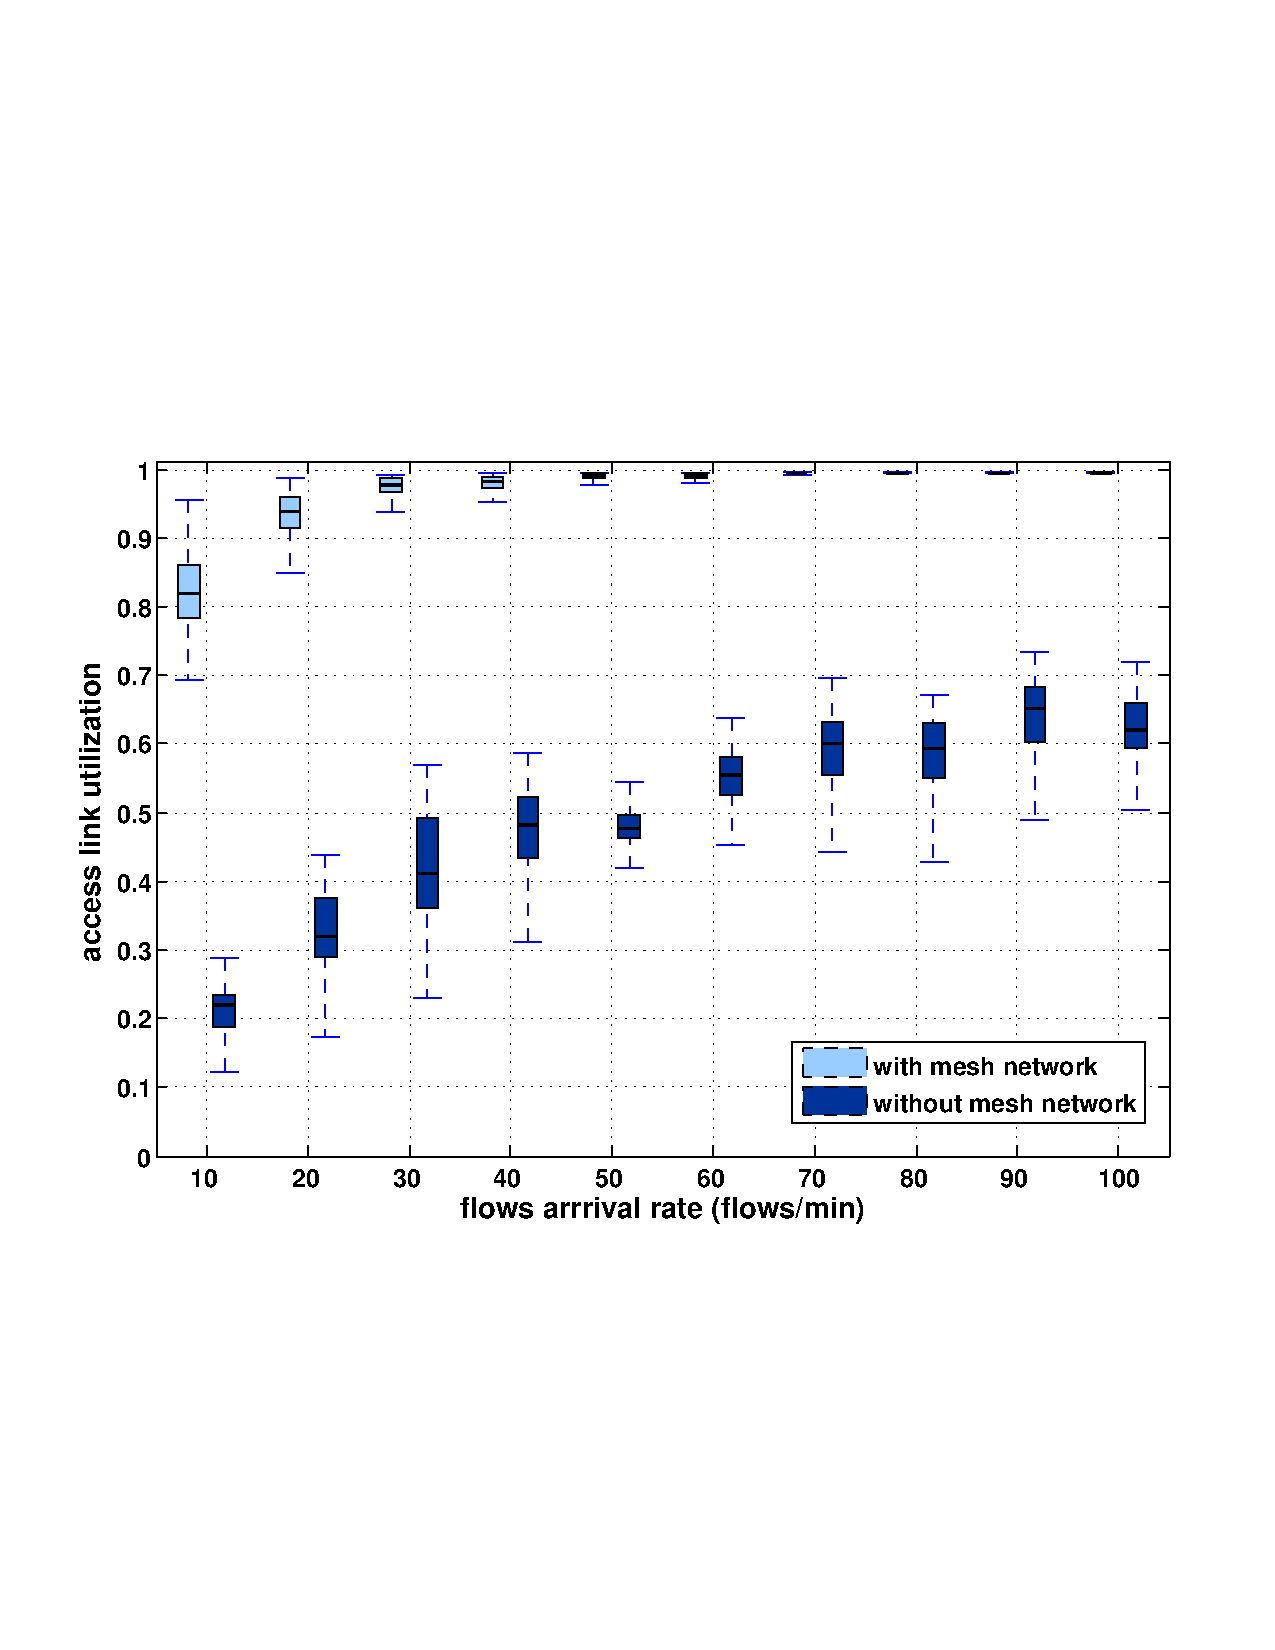
\includegraphics[width=1\linewidth]{../../results/simulation/boxplot2.pdf}  
\caption{Shared bandwidth utilization vs. flow arrival rate.}
\label{fig:utilization_arrival}
\end{center}
\end{figure}


